%% bare_conf.tex
%% V1.3
%% 2007/01/11
%% by Michael Shell
%% See:
%% http://www.michaelshell.org/
%% for current contact information.
%%
%% This is a skeleton file demonstrating the use of IEEEtran.cls
%% (requires IEEEtran.cls version 1.7 or later) with an IEEE conference paper.
%%
%% Support sites:
%% http://www.michaelshell.org/tex/ieeetran/
%% http://www.ctan.org/tex-archive/macros/latex/contrib/IEEEtran/
%% and
%% http://www.ieee.org/

%%*************************************************************************
%% Legal Notice:
%% This code is offered as-is without any warranty either expressed or
%% implied; without even the implied warranty of MERCHANTABILITY or
%% FITNESS FOR A PARTICULAR PURPOSE! 
%% User assumes all risk.
%% In no event shall IEEE or any contributor to this code be liable for
%% any damages or losses, including, but not limited to, incidental,
%% consequential, or any other damages, resulting from the use or misuse
%% of any information contained here.
%%
%% All comments are the opinions of their respective authors and are not
%% necessarily endorsed by the IEEE.
%%
%% This work is distributed under the LaTeX Project Public License (LPPL)
%% ( http://www.latex-project.org/ ) version 1.3, and may be freely used,
%% distributed and modified. A copy of the LPPL, version 1.3, is included
%% in the base LaTeX documentation of all distributions of LaTeX released
%% 2003/12/01 or later.
%% Retain all contribution notices and credits.
%% ** Modified files should be clearly indicated as such, including  **
%% ** renaming them and changing author support contact information. **
%%
%% File list of work: IEEEtran.cls, IEEEtran_HOWTO.pdf, bare_adv.tex,
%%                    bare_conf.tex, bare_jrnl.tex, bare_jrnl_compsoc.tex
%%*************************************************************************

% *** Authors should verify (and, if needed, correct) their LaTeX system  ***
% *** with the testflow diagnostic prior to trusting their LaTeX platform ***
% *** with production work. IEEE's font choices can trigger bugs that do  ***
% *** not appear when using other class files.                            ***
% The testflow support page is at:
% http://www.michaelshell.org/tex/testf low/



% Note that the a4paper option is mainly intended so that authors in
% countries using A4 can easily print to A4 and see how their papers will
% look in print - the typesetting of the document will not typically be
% affected with changes in paper size (but the bottom and side margins will).
% Use the testflow package mentioned above to verify correct handling of
% both paper sizes by the user's LaTeX system.
%
% Also note that the "draftcls" or "draftclsnofoot", not "draft", option
% should be used if it is desired that the figures are to be displayed in
% draft mode.
%
\documentclass[letterpaper, 10pt, conference, compsocconf]{IEEEtran}
% Add the compsocconf option for Computer Society conferences.
%
% If IEEEtran.cls has not been installed into the LaTeX system files,
% manually specify the path to it like:
% \documentclass[conference]{../sty/IEEEtran}



%%%%%
%TRY FIXING BY REMOVING PACKAGES INDIVIDUALLY UNTIL IT WORKS???
%%%%%

%%%%%%%%%%%%%%%%%%%%%%%%%%%%
%                          %
% Modified by Songmin Kim  %
%     Date: 20/10/15       %
%                          %
%%%%%%%%%%%%/%%%%%%%%%%%%%%%

% Basic package
\usepackage{amsmath}							% for math
\usepackage{amssymb, mathtools}					% for mathematics
\usepackage[margin=1in]{geometry}				% for page size and margins
%\usepackage{caption}							% for captions: Warning 
\usepackage{graphicx, epsfig}					% for graphics
\usepackage[tight,footnotesize]{subfigure}
\usepackage[caption=false,font=footnotesize]{subfig}
\usepackage{pdflscape, pdfpages, ifpdf}			% for pdfs
\usepackage{latexsym}							% for symbols
\usepackage{tabularx, multirow}		 			% for tables 1
\usepackage{threeparttable, longtable, tabu}	% for tables2
\usepackage{setspace}							% for line spaces
\usepackage{comment}							% for multi-line comments
\usepackage{todonotes}							% for notes
\usepackage{breqn} 								% for auto line breaks
\usepackage{xspace}								% for spacing
\usepackage[noend]{algpseudocode}				% for psudocodes
\usepackage{algorithm, algorithmicx}			% for algorithm
%\usepackage{algorithmic}						% for algorithm
\usepackage{array}								% for array
\usepackage{mdwmath,mdwtab}						% to format equations
\usepackage{eqparbox}							% for natural width parboxes
\usepackage{cite}								% for citations
\usepackage{url}								% for URL links
%\usepackage{fixltx2e}
\usepackage{stfloats}


% Style
\interdisplaylinepenalty=2500
\hyphenation{op-tical net-works semi-conduc-tor} % correct bad hyphenation here

% *** GRAPHICS RELATED PACKAGES ***
\ifCLASSINFOpdf
  % \usepackage[pdftex]{graphicx}
  % declare the path(s) where your graphic files are
  % \graphicspath{{../pdf/}{../jpeg/}}
  % and their extensions so you won't have to specify these with
  % every instance of \includegraphics
  % \DeclareGraphicsExtensions{.pdf,.jpeg,.png}
\else
  % or other class option (dvipsone, dvipdf, if not using dvips). graphicx
  % will default to the driver specified in the system graphics.cfg if no
  % driver is specified.
  % \usepackage[dvips]{graphicx}
  % declare the path(s) where your graphic files are
  % \graphicspath{{../eps/}}
  % and their extensions so you won't have to specify these with
  % every instance of \includegraphics
  % \DeclareGraphicsExtensions{.eps}
\fi

% *** Do not adjust lengths that control margins, column widths, etc. ***
% *** Do not use packages that alter fonts (such as pslatex).         ***
% There should be no need to do such things with IEEEtran.cls V1.6 and later.
% (Unless specifically asked to do so by the journal or conference you plan
% to submit to, of course. )

\begin{document}
 
% paper title
% can use linebreaks \\ within to get better formatting as desired
\title{Some\\ Title}


% author names and affiliations
% use a multiple column layout for up to two different
% affiliations

\author{\IEEEauthorblockN{Jane Doe\hspace*{0.4in}}
\IEEEauthorblockA{Information and Computer Sciences Department\\
University of Hawai`i at M\=anoa, Honolulu, HI, U.S.A.\\
$[$janedoe$]$@hawaii.edu}
%\and
%\IEEEauthorblockN{Authors Name/s per 2nd Affiliation (Author)}
%\IEEEauthorblockA{line 1 (of Affiliation): dept. name of organization\\
%line 2: name of organization, acronyms acceptable\\
%line 3: City, Country\\
%line 4: Email: name@xyz.com}
}

% conference papers do not typically use \thanks and this command
% is locked out in conference mode. If really needed, such as for
% the acknowledgment of grants, issue a \IEEEoverridecommandlockouts
% after \documentclass

% for over three affiliations, or if they all won't fit within the width
% of the page, use this alternative format:
% 
%\author{\IEEEauthorblockN{Michael Shell\IEEEauthorrefmark{1},
%Homer Simpson\IEEEauthorrefmark{2},
%James Kirk\IEEEauthorrefmark{3}, 
%Montgomery Scott\IEEEauthorrefmark{3} and
%Eldon Tyrell\IEEEauthorrefmark{4}}
%\IEEEauthorblockA{\IEEEauthorrefmark{1}School of Electrical and Computer Engineering\\
%Georgia Institute of Technology,
%Atlanta, Georgia 30332--0250\\ Email: see http://www.michaelshell.org/contact.html}
%\IEEEauthorblockA{\IEEEauthorrefmark{2}Twentieth Century Fox, Springfield, USA\\
%Email: homer@thesimpsons.com}
%\IEEEauthorblockA{\IEEEauthorrefmark{3}Starfleet Academy, San Francisco, California 96678-2391\\
%Telephone: (800) 555--1212, Fax: (888) 555--1212}
%\IEEEauthorblockA{\IEEEauthorrefmark{4}Tyrell Inc., 123 Replicant Street, Los Angeles, California 90210--4321}}




% use for special paper notices
%\IEEEspecialpapernotice{(Invited Paper)}




% make the title area
\maketitle


\begin{abstract}
This is where the abstract goes
\end{abstract}

%\begin{IEEEkeywords}
%Some keywords
%\end{IEEEkeywords}


% For peer review papers, you can put extra information on the cover
% page as needed:
% \ifCLASSOPTIONpeerreview
% \begin{center} \bfseries EDICS Category: 3-BBND \end{center}
% \fi
%
% For peerreview papers, this IEEEtran command inserts a page break and
% creates the second title. It will be ignored for other modes.
\IEEEpeerreviewmaketitle

\section{Introduction}


Lorem Ipsum is simply dummy text of the printing and typesetting industry. Lorem Ipsum has been the
industry's standard dummy text ever since the 1500s, when an unknown printer took a galley of type
and scrambled it to make a type specimen book. It has survived not only five centuries, but also the
leap into electronic typesetting, remaining essentially unchanged. It was popularised in the 1960s
with the release of Letraset sheets containing Lorem Ipsum passages, and more recently with desktop
publishing software like Aldus PageMaker including versions of Lorem Ipsum.

Contrary to popular belief, Lorem Ipsum is not simply random text. It has roots in a piece of
classical Latin literature from 45 BC, making it over 2000 years old. Richard McClintock, a Latin
professor at Hampden-Sydney College in Virginia, looked up one of the more obscure Latin words,
consectetur, from a Lorem Ipsum passage, and going through the cites of the word in classical
literature, discovered the undoubtable source. Lorem Ipsum comes from sections 1.10.32 and 1.10.33
of "de Finibus Bonorum et Malorum" (The Extremes of Good and Evil) by Cicero, written in 45 BC. This
book is a treatise on the theory of ethics, very popular during the Renaissance. The first line of
Lorem Ipsum, "Lorem ipsum dolor sit amet..", comes from a line in section 1.10.32.

The standard chunk of Lorem Ipsum used since the 1500s is reproduced below for those interested. 
Sections 1.10.32 and 1.10.33 from "de Finibus Bonorum et Malorum" by Cicero are also reproduced in
their exact original form, accompanied by English versions from the 1914 translation by H. Rackham.

Check out Table~\ref{tab:sometable}.

\begin{table}[ht]
\caption{Some caption}
\label{tab:sometable}
\centering
\begin{tabular}{|l|c|}
\hline
hello & foo \\
bar & bye\\
\hline
\end{tabular}
\end{table}

\subsection{Some Subsection}

See stuff in Figure~\ref{fig:somefig}. It's a \textcolor{red}{cow}!

And I can even do math!
$$
\sum_{i=1}^n i = \frac{n (n+1)}{2}
$$

\begin{figure}[t]
\centering
  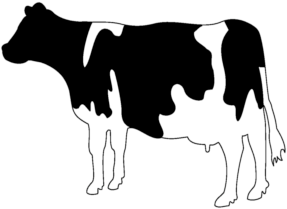
\includegraphics[width=0.4\textwidth]{fig/cow.pdf}  
    \caption{Some caption.}
   \label{fig:somefig}
\end{figure}

\subsection{Some Subsection}

\section{Some Other Section}

Here is a bibliographical reference~\cite{somepaper}.

\section{Conclusion}

\bibliographystyle{IEEEtran}
\bibliography{biblio} 


\end{document}


